%%%%%%%%%%%%%%%%%%%%%%%%%%%%%%%%%%%%%%%%%%%%%%%%%%%%%%%%%%%%%%%%%%%%%%%%%%%%%%%%%%%%%%%%%%%%%%%%%%%%%%%%%%%%%%%%%%%%%%%%%%%%%%%%%
\chapter{Implementation on the Server Side}
\label{cha:on_the_server_side}

In order to retrieve information about nearby stops, the client must request a remote source of information by calling a server. The server that has been implemented in our case acts as a middle-ware between the public transport providers (Västtrafik and SL) and the client. In that way, requests to the different providers are transparent to the client.

%%%%%%%%%%%%%%%%%%%%%%%%%%%%%%%%%%%%%%%%%%%%%%%%%%%%%
\section{Architecture}

The server processes a request for nearby bus stops as follows:

\begin{enumerate}
\item{receive a request with the user's coordinates (Latitude and Longitude),}
\item{find the 10 nearest bus locations from the given coordinates in its SQLite database,}
\item{for each of these stops, launch a light-weighted process that:
\begin{enumerate}
	\item{if valid cached data is available in its Mnesia database, returns this data as forecast}
	\item{otherwise, fetch forecast data from the stop's provider}
\end{enumerate}
}
\item{once each forecast is obtained, parse the result into JSON format,}
\item{finally, send a reply to the client containing the JSON data.}
\end{enumerate}

Figure \ref{fig:message_passing} shows a simplified request processing on an UML sequential diagram, the grey area representing our server. The sequence is simplified because it describes a process that only returns three stops instead of ten, plus it does not explicitly shows the caching mechanism, but it is still a good representation of what is happening.\\
\clearpage
\begin{figure}[ht]
\center
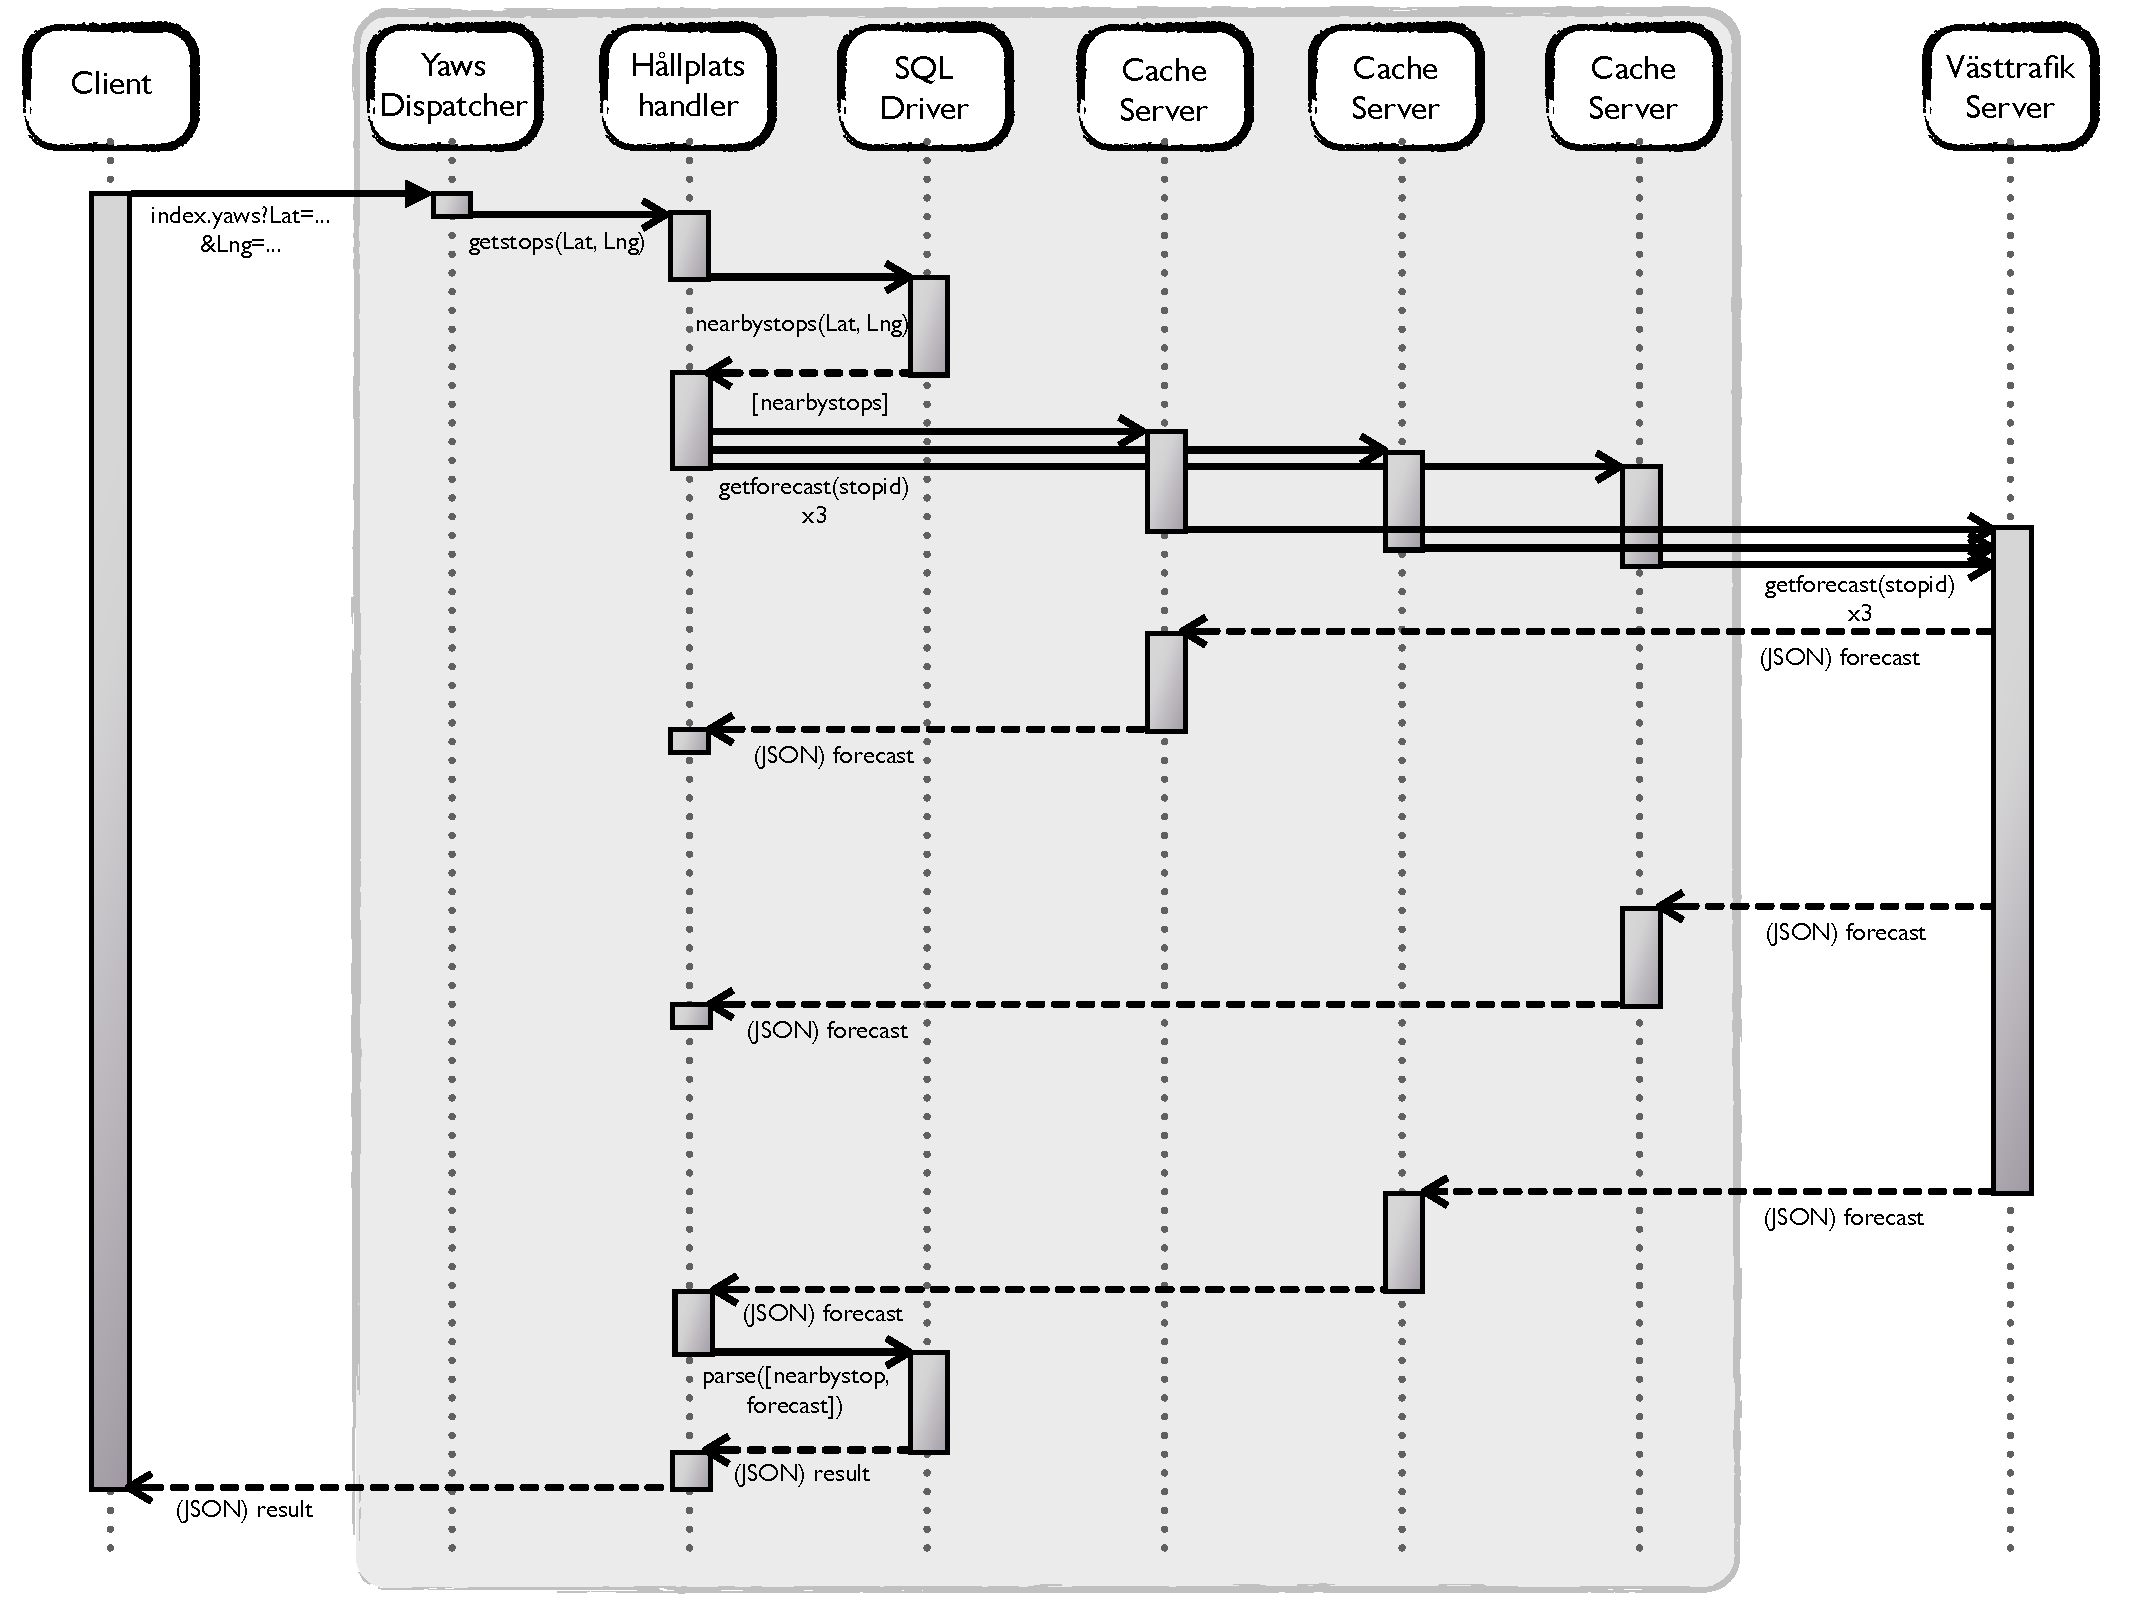
\includegraphics[scale=0.4]{pics/message_passing}
\caption{UML sequential diagram of the request processing}
\label{fig:message_passing}
\end{figure}

This diagram follows the classic UML notation, so plain arrows represent synchronous calls, stick arrows represent asynchronous calls, and dashed arrows represent return values. \\

The application is hosted on a Yaws web server installed on a Debian (Ubuntu) virtual machine from the Amazon cloud web services. Yaws is the Erlang alternative to web servers, and as such offers high availability and high scalability.\\

In order to handle high quantities of lightweight processes, the best solution was to use Erlang. Erlang is a functional programming language especially designed to handle high concurrency and distributed systems.  A large part of the application is therefore implemented in Erlang in order to take advantage of this \label{sec:erlang_intro}.\\

But to keep the application easy to maintain and update, the more complex tasks are implemented in Ruby. Ruby is a modern dynamic scripted language, and has been designed to make the developers happy. As such, it is a powerful tool to implement complex algorithms painlessly. The ruby part is hosted on a rails web server, and communicates with the Yaws server through Erlang Ports via the Erlang Binary Protocol.\\

Figure \ref{fig:server_architecture} shows the details of the server's architecture.\\

\begin{figure}[ht]
\center
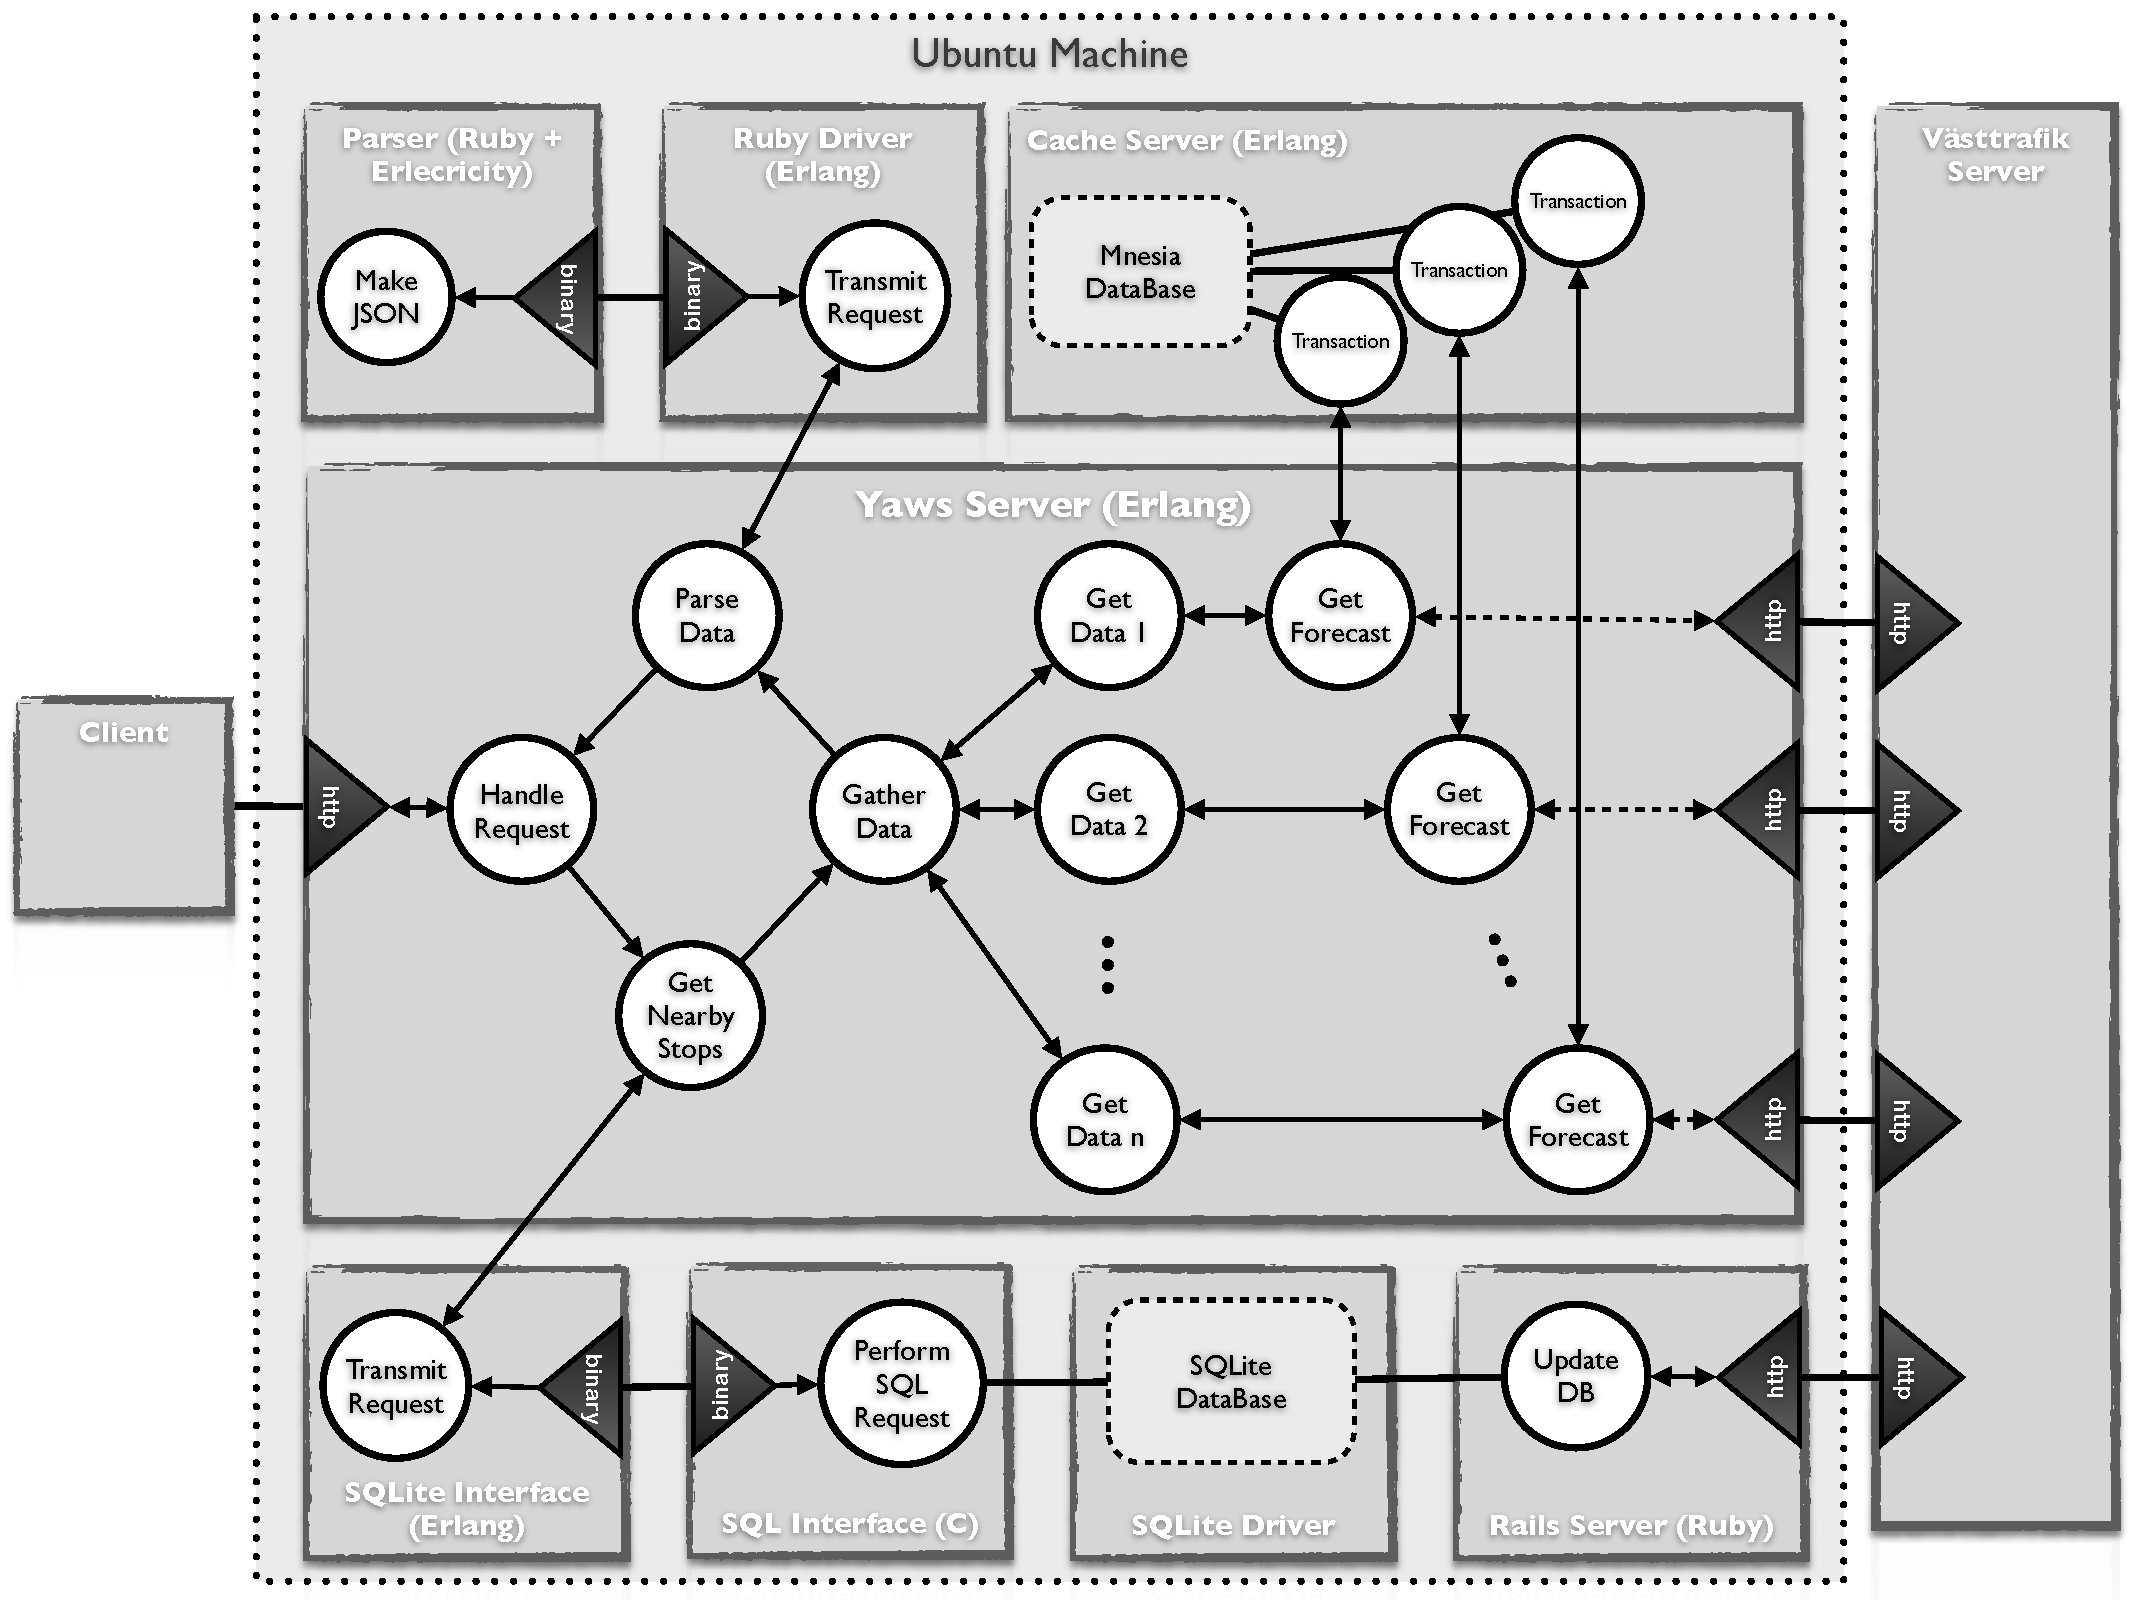
\includegraphics[scale=0.4]{pics/server_side}
\caption{Scheme of the Server Architecture}
\label{fig:server_architecture}
\end{figure}

In this figure, each circle represents an independent process and the arrows indicate message passing between processes. The dashed rounded rectangles represent databases servers. Black triangles represent communication ports.

\clearpage
%%%%%%%%%%%%%%%%%%%%%%%%%%%%%%%%%%%%%%%%%%%%%%%%%%%%%
\section{Erlang}

Erlang is used to dispatch the lightweight processes, to query the SQLite database, to perform the distant requests to Västtrafik and Storstockholms Locaktrafik, but also to take care of data caching via a Mnesia database. This obviously represents the larger part of the server's application.\\

The complete implementation of the Erlang parts is given in Appendix \ref{cha:erlang}.

\subsection{Concurrent Programming}

As mentioned in Section \ref{sec:erlang_intro}, Erlang is a functional language, and as such differs greatly from classic programming paradigms. In Erlang, functions are treated in a pure mathematical way: variables are immutable and functions have no side effects. This may seems like a very handicapping restriction, but that is what makes Erlang so powerful at smoothly handling thousands of concurrent processes without having problems of dead locks, starvation nor memory corruption.\\

Being a functional language, Erlang allows function recursion with very little overhead. It also feature strong pattern matching capabilities. The piece of code shown in Figure \ref{fig:erlang_factorial} is an implementation of the factorial function programmed in Erlang.\\

\begin{figure}[ht]
  \centering
  \fbox{ 
    \colorbox{light-gray}{
      \begin{minipage}{12cm}
        \small{\begin{Verbatim}[commandchars=@\[\]]
-@PYay[module](example).
-@PYay[export](@PYZlb[]factorial@PYbf[/]@PYag[1]@PYZrb[]).

@PYaL[factorial](@PYag[0]) @PYbf[-]@PYbf[>]
    @PYag[1];
@PYaL[factorial](@PYaj[N]) @PYbf[-]@PYbf[>]
    @PYaj[N] @PYbf[*] factorial(@PYaj[N]@PYbf[-]@PYag[1]).
\end{Verbatim}
}
      \end{minipage}
    }
  }
  \caption{Implementation of the factorial function in Erlang}
  \label{fig:erlang_factorial}
\end{figure}

From this snippet we can see that the Erlang implementation is very close to the mathematical definition of factorial:

 \[n! = 
            \left\{
              \begin{array}{l l}
                   1 & \textrm{if } n = 0\\
                   n \times (n - 1)! & \textrm{otherwise}
               \end{array}
            \right.
\] 

This is made possible thanks to pattern matching, and it is efficient thanks to tail recursion optimization.\\

But the real power of Erlang reside in its messaging system that allows complex asynchronous calls. When a process sends a message to another process, the message is put into the receiver's message box to be treated whenever it is available. By doing so, message passing is a totally non blocking procedure.\\

\begin{figure}[ht]
  \centering
  \fbox{ 
    \colorbox{light-gray}{
      \begin{minipage}{12cm}
        \small{\begin{Verbatim}[commandchars=@\[\]]
-@PYay[module](example).
-@PYay[export](@PYZlb[]start@PYbf[/]@PYag[0], ping@PYbf[/]@PYag[0]@PYZrb[]).

@PYaL[ping]() @PYbf[-]@PYbf[>]
  @PYaz[receive]
    {ping, @PYaj[Pong_PID]} @PYbf[-]@PYbf[>]
      @PYaW[io]:format(@PYad["]@PYad[Ping!]@PYbg[~n]@PYad["], @PYZlb[]@PYZrb[]),
      @PYaj[Pong_PID]@PYbf[!]pong,
      ping()
  @PYaz[end].

@PYaL[start]() @PYbf[-]@PYbf[>]
  @PYaj[Ping_PID] @PYbf[=] @PYaY[spawn](example, ping, @PYZlb[]@PYZrb[]),
  @PYaj[Ping_PID]@PYbf[!]{ping, self()},
  @PYaz[receive]
    {pong} @PYbf[-]@PYbf[>]
      @PYaW[io]:format(@PYad["]@PYad[Pong!]@PYbg[~n]@PYad["], @PYZlb[]@PYZrb[])
  @PYaz[end].
\end{Verbatim}
}
      \end{minipage}
    }
  }
  \caption{Simple example of message passing in Erlang}
  \label{fig:erlang_message}
\end{figure}

Figure \ref{fig:erlang_message} shows a simple message passing procedure between two processes. The "spawn" command spawns a new process with the function passed as its argument, then returns its Process ID (PID). To send a message to a process, one must use the "!" command preceded by the PID of the receiver and followed by the message to be sent. The "self()" function returns the PID of the current process, so if an answer is required from the contacted process, one can pass its own PID along with the message it sends. The "receive" block is defined to handle received messages matching the supported messages.\\

Erlang has many more features that could not be treated in this paper such as list comprehension or hot code swapping, but more information can be easily found on the Internet \cite{Erl10}.

\subsection{Port Communication}

In our implementation, we need Erlang to communicate with Ruby. To do so, one can open a communication "Port" in Erlang that will maintain a link to an external driver, in our case a ruby script (See Figure \ref{fig:erlang_port}). The Port will be kept open as long as a process is linked to it, so in our case we spawn a process that will act as a server to the Ruby port.\\

\begin{figure}[ht]
  \centering
  \fbox{ 
    \colorbox{light-gray}{
      \begin{minipage}{12cm}
        \small{\begin{Verbatim}[commandchars=@\[\]]
@PYaL[start_driver]() @PYbf[-]@PYbf[>]
  @PYaj[Cmd] @PYbf[=] @PYad["]@PYad[rails runner ./lib/echo.rb]@PYad["],
  @PYaj[Port] @PYbf[=] @PYaY[open_port]({@PYaY[spawn], @PYaj[Cmd]}, @PYZlb[]{packet, @PYag[4]}, nouse_stdio,
            exit_status, binary@PYZrb[]).
\end{Verbatim}
}
      \end{minipage}
    }
  }
  \caption{Example of Port opening with Erlang}
  \label{fig:erlang_port}
\end{figure}

A Port is transparent in Erlang, so communicating through it is equivalent to talking to a local process. This is actually very powerful, because Ports are typically bridges between servers, so distant and local process communications are perfectly identical.\\

An Erlang port is also opened in the same fashion to perform requests to the SQLite database.

\subsection{Mnesia}

The standard database to be used with Erlang is Mnesia. With Mnesia, Erlang records represent key-value tuples where the value can be any data structure, from simple integer to Erlang lambda functions.\\

The query language to the database is Erlang itself and not a third party language such as SQL, which enable all the features of Erlang within the request procedure: pattern matching and list comprehension among others. To perform a query, one must perform a "transaction". A transaction will ensure that any read/write procedure to the database is performed properly. Transactions can easily be nested and can also be distributed on different process/servers transparently. A simple query example is shown in Figure \ref{fig:mnesia_example}.\\

\begin{figure}[ht]
  \centering
  \fbox{ 
    \colorbox{light-gray}{
      \begin{minipage}{12cm}
        \small{\begin{Verbatim}[commandchars=@\[\]]
@PYaL[all_females]() @PYbf[-]@PYbf[>]
  @PYaj[F] @PYbf[=] @PYaz[fun]() @PYbf[-]@PYbf[>]
      @PYaj[Female] @PYbf[=] @PYai[#employee]{sex @PYbf[=] female, name @PYbf[=] '$1', _ @PYbf[=] '_'},
      @PYaW[mnesia]:select(employee, @PYZlb[]{@PYaj[Female], @PYZlb[]@PYZrb[], @PYZlb[]'$1'@PYZrb[]}@PYZrb[])
      @PYaz[end],
  @PYaW[mnesia]:transaction(@PYaj[F]).
\end{Verbatim}
}
      \end{minipage}
    }
  }
  \caption{Simple example of query to Mnesia Database returning the names of all female employees}
  \label{fig:mnesia_example}
\end{figure}

Our implementation of the cache server uses Mnesia to store cached data. The database only has one table containing the pairs of key-values corresponding to "url", "data" and "timestamp". The URL is used as an index for queries to the database, and the timestamp is here to check when the cached data should expire.\\

More information about Mnesia can be found on the Internet \cite{Mne10}.

\section{SQLite}

Mnesia is very powerful and fast, but it can only be accessible via Erlang. This makes it an inappropriate choice for a database that requires maintenance or arbitrary updates. On the contrary, SQLite is a very convenient database accessible in virtually any language, particularly Erlang in Ruby in our case.\\

By querying the SQLite database with Erlang while maintaining it with Ruby makes the application efficient and yet easy to maintain.\\

The SQLite database contains information on all the bus stops for each provider. Each entry in the database has the following attributes:\\

\begin{tabular}{ l l l l }
$\bullet$ & stop\_name 	& : & the name of the stop\\
$\bullet$ & lat 			& : & the Latitude of the stop\\
$\bullet$ & lng 			& : & the Longitude of the stop\\
$\bullet$ & provider\_name & : & the name of the stop's provider (Västtrafik or SL)\\
$\bullet$ & stop\_id 		& : & the id of the stop as defined by its provider\\
$\bullet$ & timestamp 	& : & the timestamp of the stop creation\\
$\bullet$ & id		 	& : & a unique ID for indexing\\
\end{tabular}\\

\clearpage
The "lat" and "lng" attributes are the key entries allowing geographic search in the database, but finding nearby points from a database can be a tricky problem. In our case, we perform queries iteratively as shown in Figure \ref{fig:ruby_queries} until a satisfying number of stops are returned.\\

\begin{figure}[ht]
\center
\subfigure[Step 1]{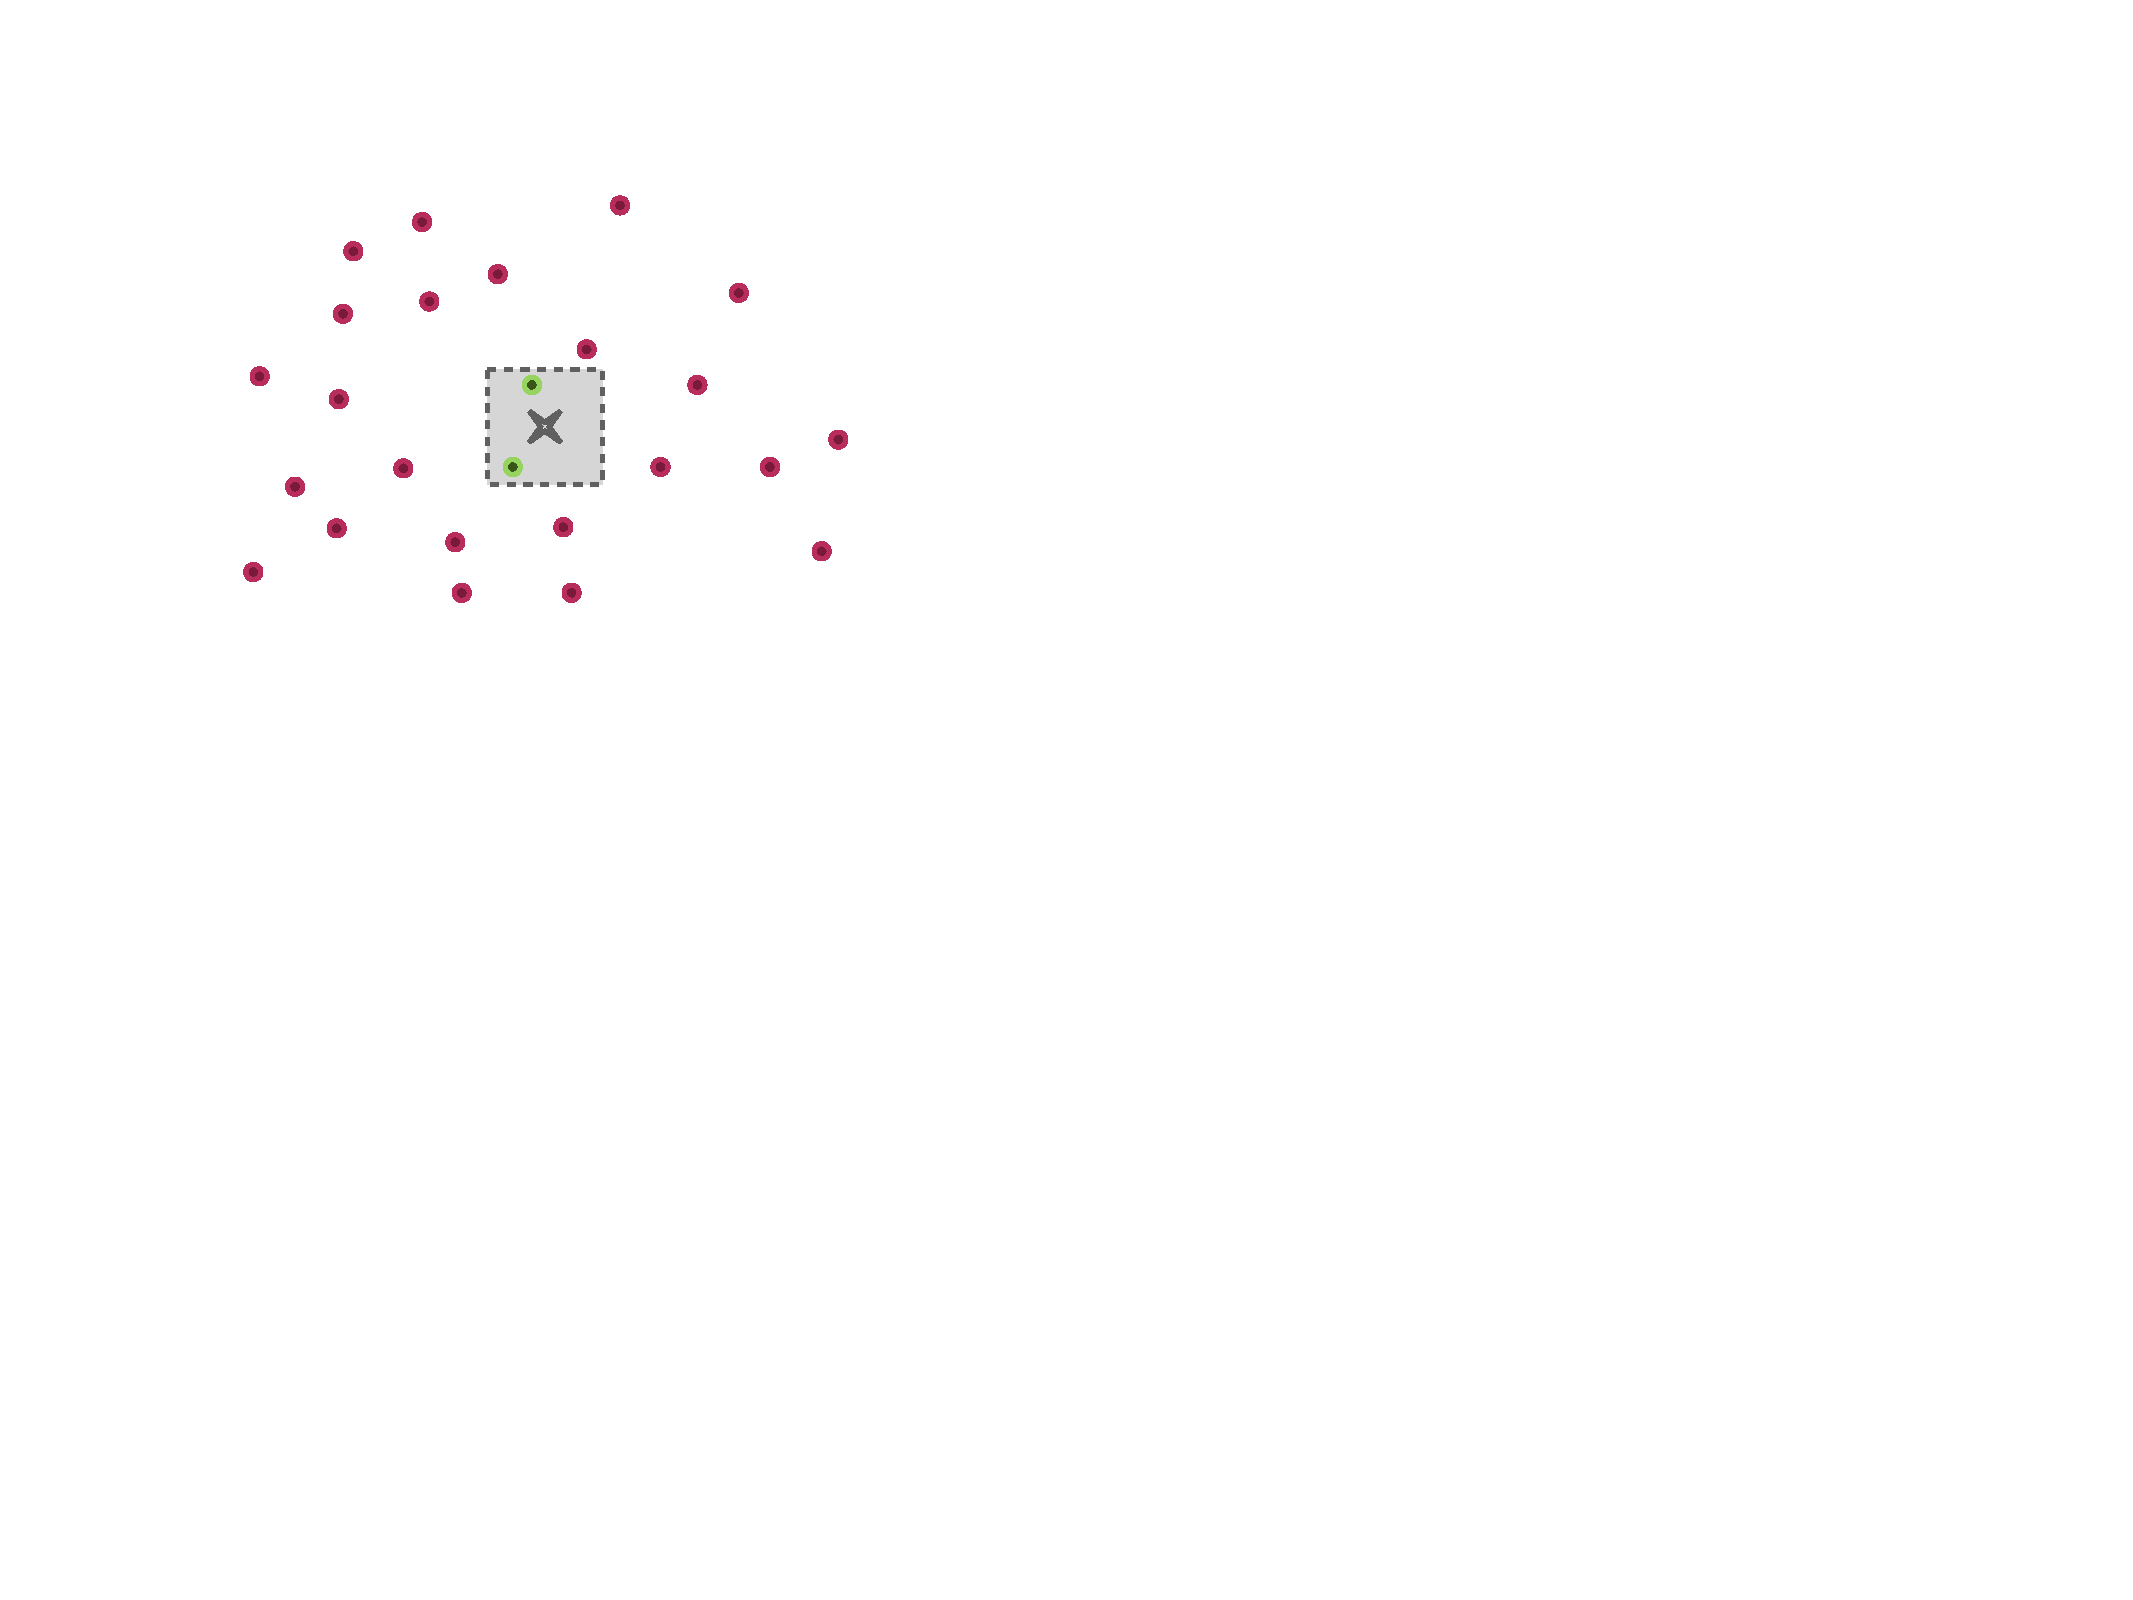
\includegraphics[scale=0.33]{pics/ruby_query_1}}
\subfigure[Step 2]{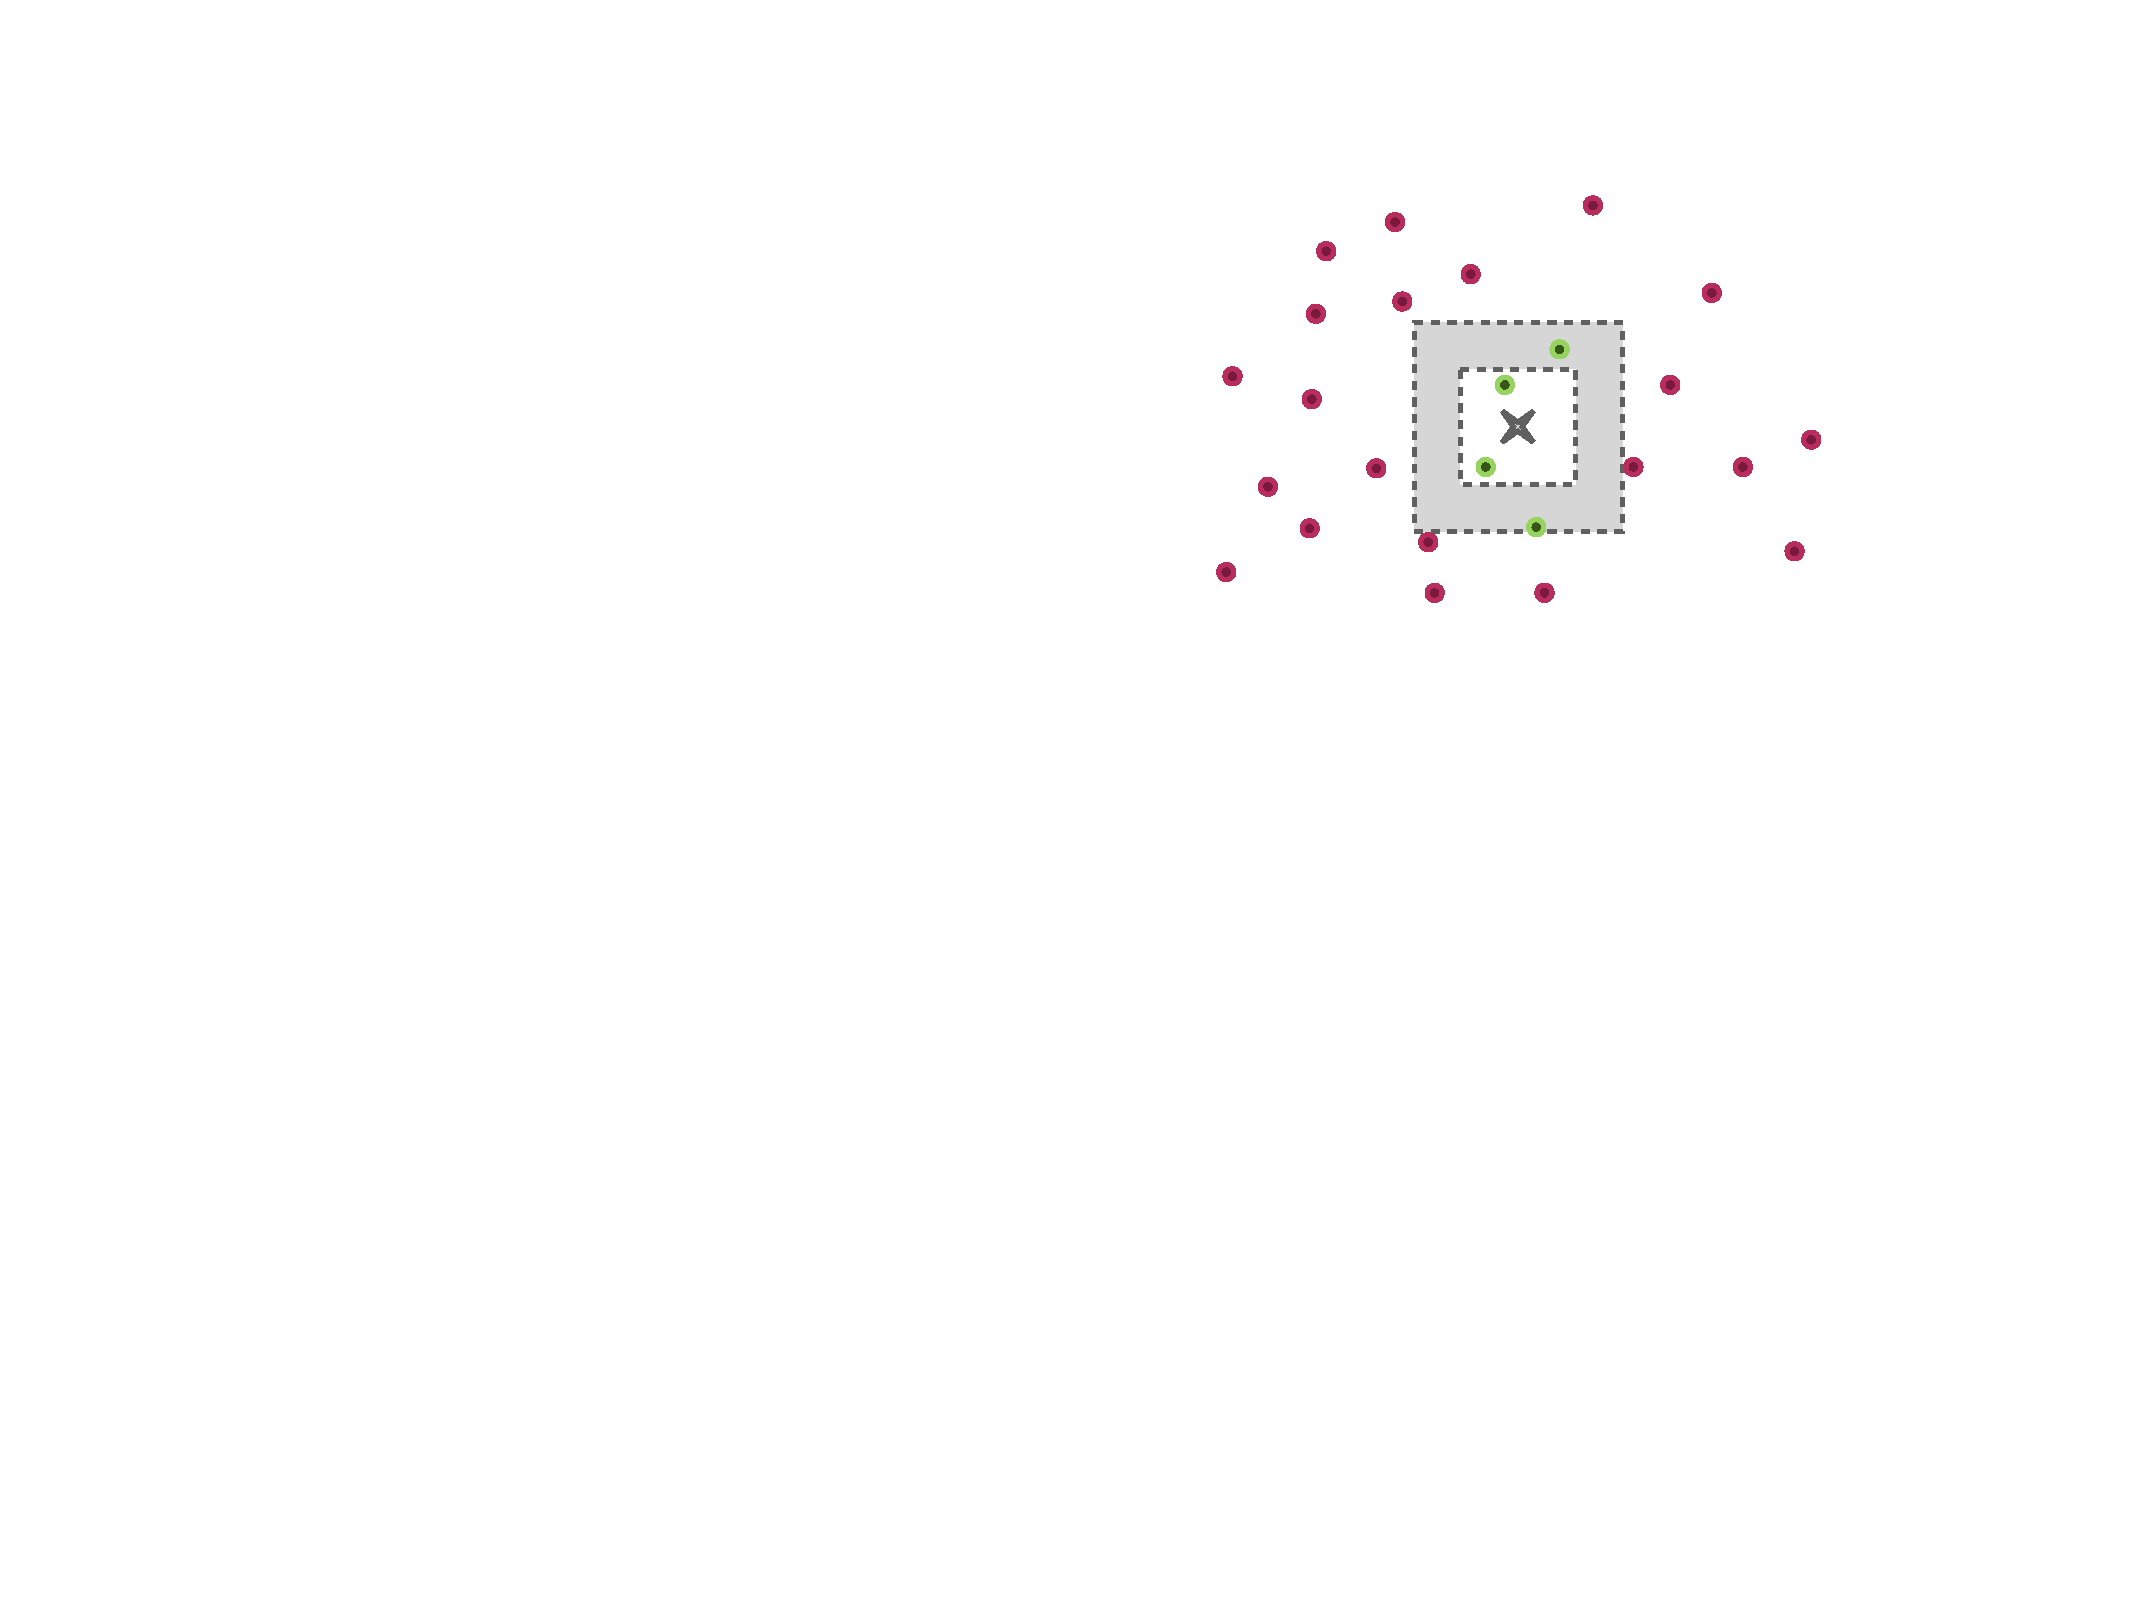
\includegraphics[scale=0.33]{pics/ruby_query_2}}
\subfigure[Step 3]{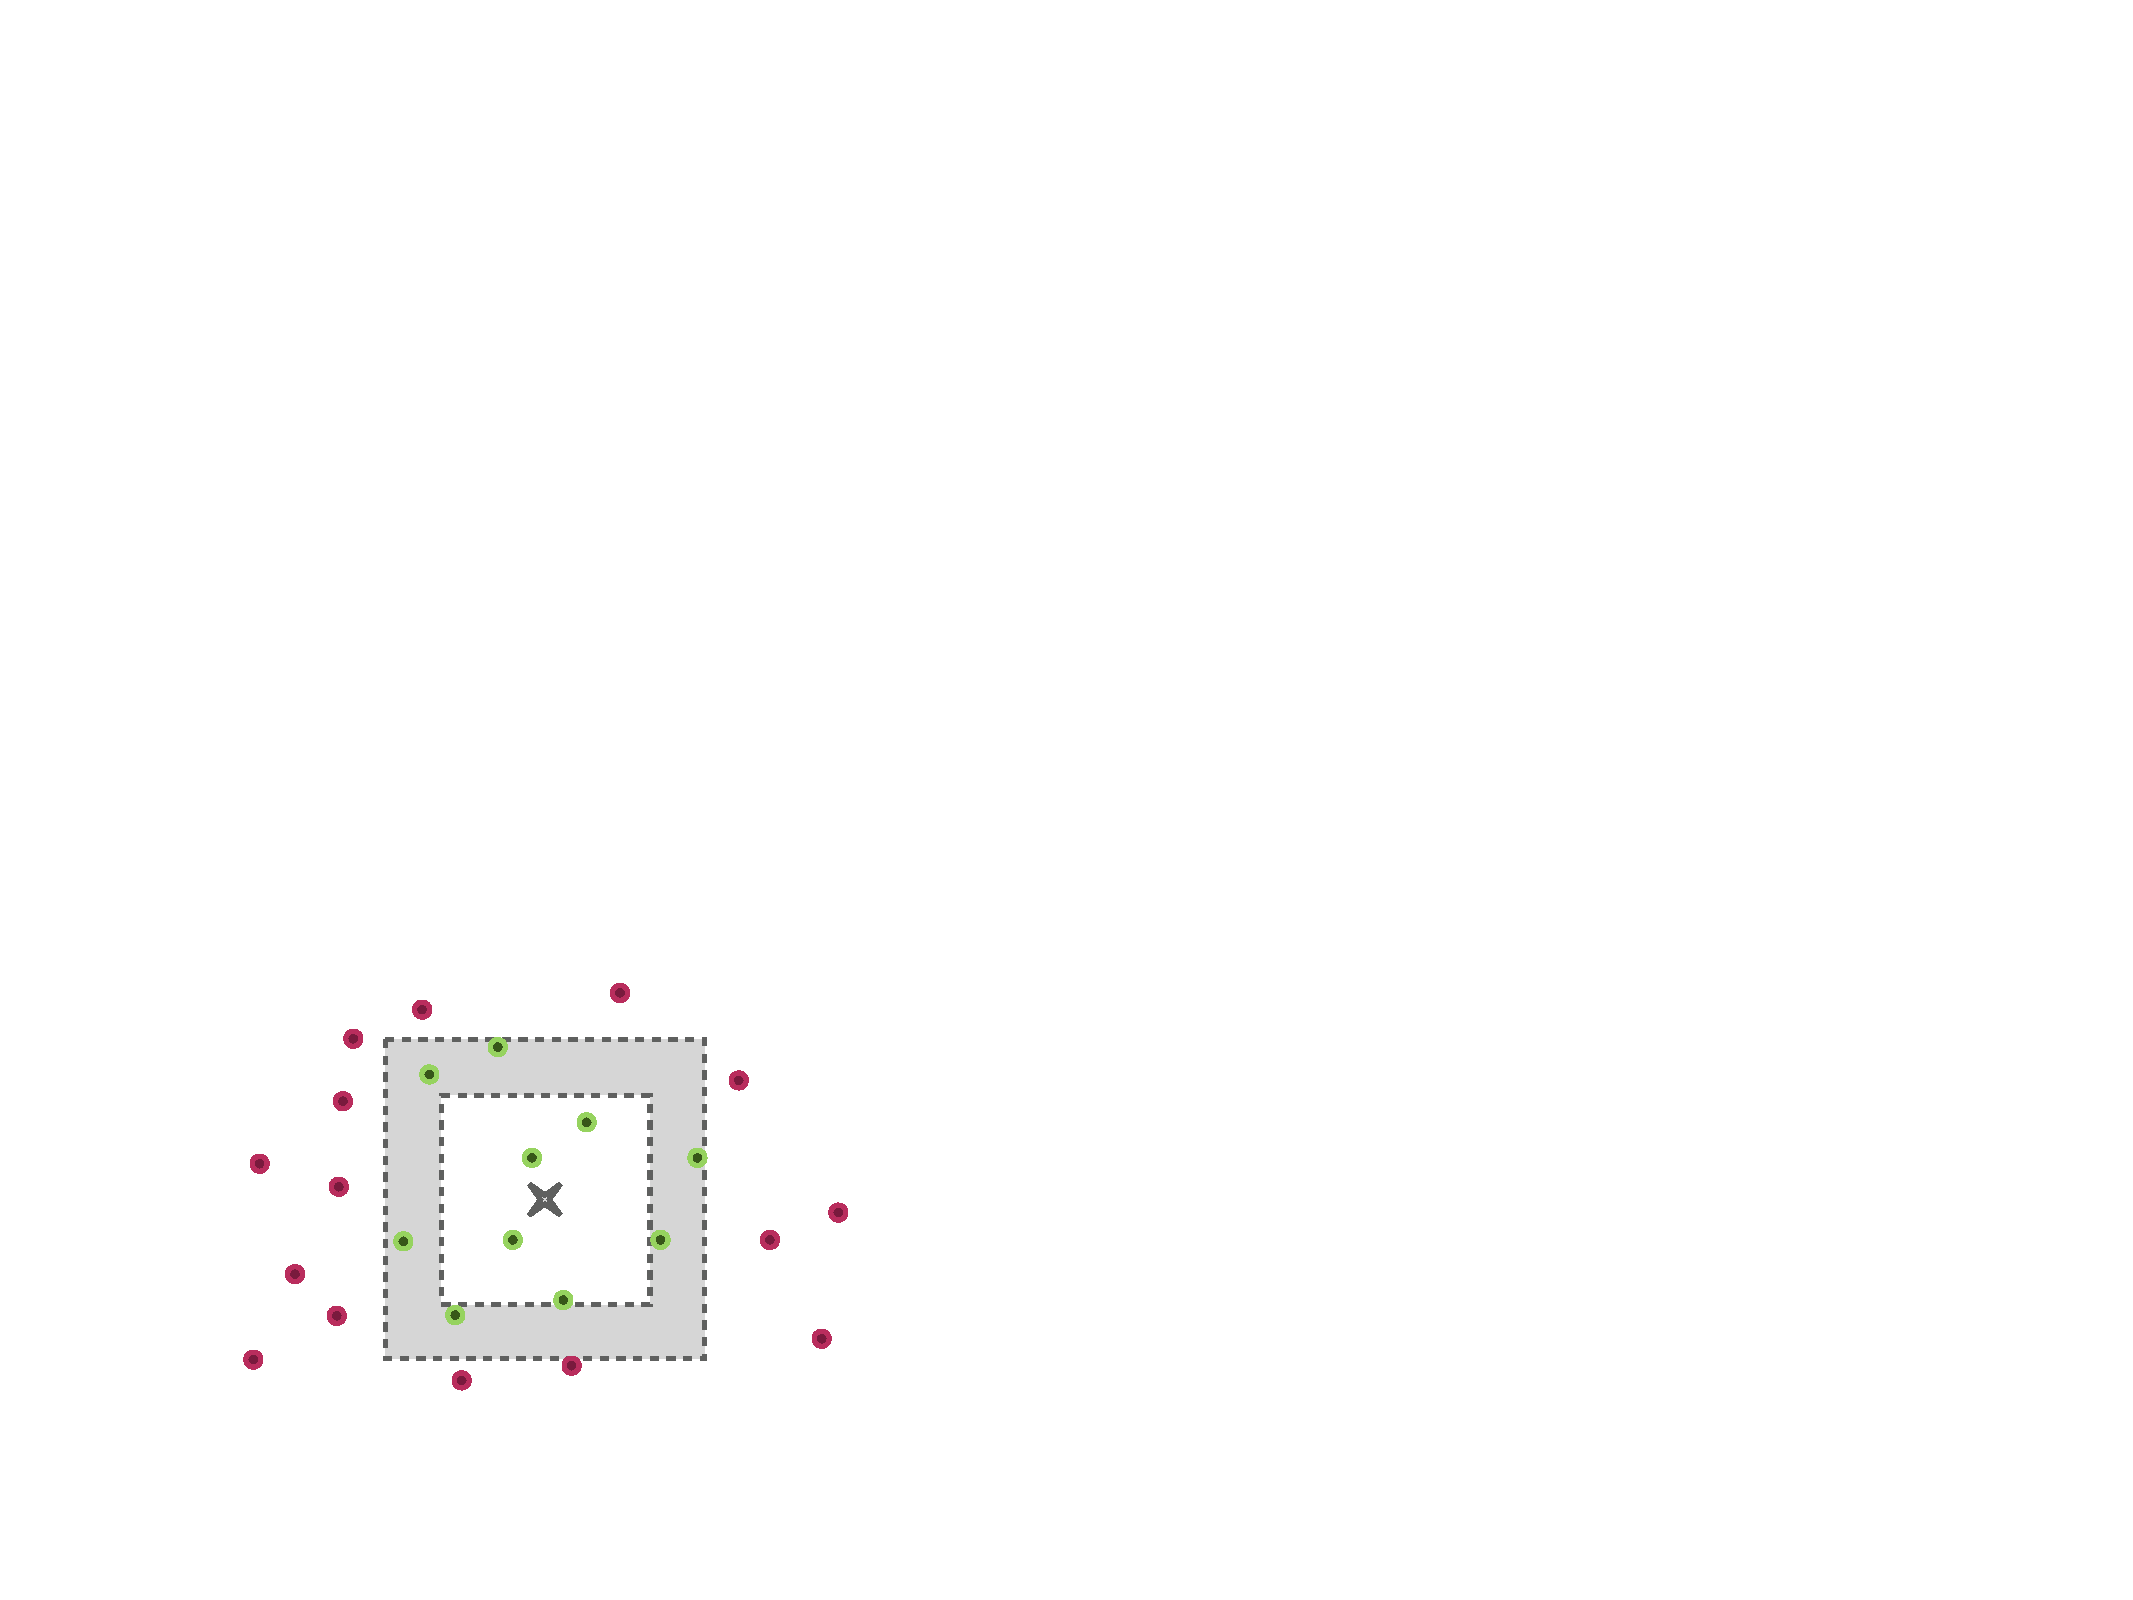
\includegraphics[scale=0.33]{pics/ruby_query_3}}
\caption{Scheme of the SQL queries on the Ruby side}
\label{fig:ruby_queries}
\end{figure}

The first step consist of a SQL query is of the following form:

\parbox{15cm}{
\begin{Verbatim}[commandchars=@\[\]]
@PYaz[SELECT] @PYbf[*] @PYaz[FROM] bus_stops @PYaz[WHERE] lat @PYbf[>]@PYbf[=] lat1 @PYaz[AND]
                              lat @PYbf[<]@PYbf[=] lat2 @PYaz[AND]
                              lng @PYbf[>]@PYbf[=] lng1 @PYaz[AND]
                              lng @PYbf[<]@PYbf[=] lng2
\end{Verbatim}

}

This will return all the bus stops within the area defined by the square defined by:

\begin{equation}
(lat, lng) \in [lat_1, lat_2]\times[lng_1, lng_2]
\end{equation}

The retrieved stops are stored in a bus list. The following steps produce queries defined as follow:

\parbox{15cm}{
\begin{Verbatim}[commandchars=@\[\]]
@PYaz[SELECT] @PYbf[*] @PYaz[FROM] bus_stops @PYaz[WHERE] lat @PYbf[>]@PYbf[=] lat1 @PYaz[AND]
                              lat @PYbf[<]@PYbf[=] lat2 @PYaz[AND]
                              lng @PYbf[>]@PYbf[=] lng1 @PYaz[AND]
                              lng @PYbf[<]@PYbf[=] lng2 @PYaz[AND] @PYaz[NOT]
                                      (lat @PYbf[>] lat3 @PYaz[AND]
                                       lat @PYbf[<] lat4 @PYaz[AND]
                                       lng @PYbf[>] lng3 @PYaz[AND]
                                       lng @PYbf[<] lng4)
\end{Verbatim}

}

This will return all the bus stops within the area defined by the area defined by:
\begin{equation}
(lat, lng) \in \left([lat_1, lat_2]\times[lng_1, lng_2]\right) \backslash \left(]lat_3, lat_4[\times]lng_3, lng_4[\right)
\end{equation}

The retrieved stops are added to the stop list until the list is large enough to proceed. In our case, we stop the algorithm when the stop list has more than 10 entries.\\

Once we get a list of stops within an arbitrary large area, we need to sort those stops by distance in order to keep only the 10 closer ones. The distance $d$ between the user's location and a stop is computed according to a simplified version of the great-circle distance formula given in Equation \ref{equ:great_circle_formula}, where $\varphi_s$ and $\lambda_s$ are the Latitude and Longitude of the standpoint, $\varphi_f$ and $\lambda_f$ the ones of the forepoint, and $R$ being the average radius of Earth ($\approx6371$km).\\

\begin{equation}
\label{equ:great_circle_formula}
d =  R \times \textrm{arccos}\left(\textrm{sin}\varphi_s \textrm{ sin}\varphi_f + \textrm{cos}\varphi_s \textrm{ cos}\varphi_f \textrm{ cos}(\lambda_f-\lambda_s)\right)
\end{equation}

\section{Ruby}

Ruby is a modern dynamic object-oriented programming language in which everything is an object, exactly as the programming language Smalltalk from which it is partly inspired. It has been designed to follow the least surprise principle during development: code should never behave in an unexpected way. It is a powerful language for writing scripts and developing applications in a very productive manner.\\

The complete implementation of the Ruby parts is given in Appendix \ref{cha:ruby}.

\subsection{Setup}

Ruby comes with a package manager called RubyGems that provides a standard distribution system for libraries. A Ruby library is called a Gem.\\

Among those Gems we find Rails, a framework that allows to deploy web applications using Ruby. When creating a Rails application, a web server is packed in, and that is what we have used in our project. We worked with Rails 3.0.0beta3, the current edge version of the framework, to deploy our Ruby application.\\

An other Gem was require to implement an interface with Erlang, so we used Erlectricity \cite{Fle09}. This library enable Ruby to send messages via the Erlang Binary Protocol, making communication between the two languages transparent. Figure \ref{fig:erlectricity_example} shows a simple implementation of communication.\\

\begin{figure}[ht]
\centering
\subfigure[Ruby Side]{
  \centering
  \fbox{ 
    \colorbox{light-gray}{
      \begin{minipage}{12cm}
        \small{\begin{Verbatim}[commandchars=@\[\]]
@PYaY[require] @PYbe['rubygems']
@PYaY[require] @PYbe['erlectricity']

receive @PYaz[do] @PYbf[|]f@PYbf[|]
  f@PYbf[.]when(@PYbf[@PYZlb[]]@PYau[:echo], @PYaY[String]@PYbf[@PYZrb[]]) @PYaz[do] @PYbf[|]text@PYbf[|]
    f@PYbf[.]send!(@PYbf[@PYZlb[]]@PYau[:result], @PYaX["]@PYaX[You said: ]@PYbg[#{]text@PYbg[}]@PYaX["]@PYbf[@PYZrb[]])
    f@PYbf[.]receive_loop
  @PYaz[end]
@PYaz[end]
\end{Verbatim}
}
      \end{minipage}
    }
  }
}

\subfigure[Erlang Side]{
  \centering
  \fbox{ 
    \colorbox{light-gray}{
      \begin{minipage}{12cm}
        \small{\begin{Verbatim}[commandchars=@\[\]]
-@PYay[module](echo).
-@PYay[export](@PYZlb[]test@PYbf[/]@PYag[0]@PYZrb[]).

@PYaL[test]() @PYbf[-]@PYbf[>]
  @PYaj[Cmd] @PYbf[=] @PYad["]@PYad[ruby echo.rb]@PYad["],
  @PYaj[Port] @PYbf[=] @PYaY[open_port]({@PYaY[spawn], @PYaj[Cmd]}, @PYZlb[]{packet, @PYag[4]}, nouse_stdio,
                                     exit_status, binary@PYZrb[]),
  @PYaj[Payload] @PYbf[=] @PYaY[term_to_binary]({echo, @PYbf[<]@PYbf[<]@PYad["]@PYad[hello world!]@PYad["]@PYbf[>]@PYbf[>]}),
  @PYaY[port_command](@PYaj[Port], @PYaj[Payload]),
  @PYaz[receive]
    {@PYaj[Port], {data, @PYaj[Data]}} @PYbf[-]@PYbf[>]
      {result, @PYaj[Text]} @PYbf[=] @PYaY[binary_to_term](@PYaj[Data]),
      @PYaW[io]:format(@PYad["]@PYbg[~p]@PYbg[~n]@PYad["], @PYZlb[]@PYaj[Text]@PYZrb[])
  @PYaz[end].
\end{Verbatim}
}
      \end{minipage}
    }
  }
}
\caption{Simple example of communication between Erlang and Ruby using Erlectricity }
\label{fig:erlectricity_example}
\end{figure}

One problem that we faced when communicating between Ruby and Erlang was when dealing with strings: Erlang can only handle Latin-1 encoded strings, whereas Ruby manipulates UTF-8 strings by default. So whenever a string is sent to be treated in Erlang, it has to be encoded in Latin-1 first, and when a string is received by Ruby, it has to be converted to UTF-8.\\

It has to be mentioned that Erlang and Yaws can handle strings in an arbitrary encoding under binary form, so when answering to the client the reply is actually UTF-8 encoded.

\subsection{Database Management}

Now that we know the required setup for our Ruby Implementation, let us have a look at what we want Ruby to do for us.\\

In our server application, Ruby is used to maintain the SQLite database.  This database is populated by a background process that fetch data from the providers on monthly basis (it is not that often that new stops are build or that old one are destroyed). Updates are performed via requests to the webservices of the providers.\\

In order to perform those required maintenance processes, we make use of Rake, a Ruby-based software build tool that is packaged as a middle-ware within Ruby on Rails.\\

Rake combined with Rails offers powerful tools for database management, especially thanks to the ActiveRecord class. An Active Record object does not specify its attributes directly but infer them from the table definition with which they‘re linked. Adding, removing, and changing attributes and/or their type is done directly in the database.\\

The are different parts of the code required to set up our SQLite database are shown in Figures \ref{fig:database}, \ref{fig:create_bus_stops} and \ref{fig:bus_stop}. 

\begin{figure}[ht]
  \centering
  \fbox{ 
    \colorbox{light-gray}{
      \begin{minipage}{12cm}
        \small{\begin{Verbatim}[commandchars=@\[\]]
@PYaf[# SQLite version 3.x]
development:
  adapter: sqlite3
  database: db@PYbf[/]development@PYbf[.]sqlite3
  pool: @PYag[5]
  timeout: @PYag[5000]

@PYaY[test]:
  adapter: sqlite3
  database: db@PYbf[/]@PYaY[test]@PYbf[.]sqlite3
  pool: @PYag[5]
  timeout: @PYag[5000]

production:
  adapter: sqlite3
  database: db@PYbf[/]production@PYbf[.]sqlite3
  pool: @PYag[5]
  timeout: @PYag[5000]
\end{Verbatim}
}
      \end{minipage}
    }
  }
  \caption{Configuration file that tells how to access the database (database.yml)}
  \label{fig:database}
\end{figure}

\clearpage

\begin{figure}[ht]
  \centering
  \fbox{ 
    \colorbox{light-gray}{
      \begin{minipage}{12cm}
        \small{\begin{Verbatim}[commandchars=@\[\]]
@PYaz[class] @PYaO[CreateBusStops] @PYbf[<] @PYar[ActiveRecord]@PYbf[::]@PYar[Migration]
  @PYaz[def] @PYaO[self]@PYbf[.]@PYaL[up]
    create_table @PYau[:bus_stops] @PYaz[do] @PYbf[|]t@PYbf[|]
      t@PYbf[.]string @PYau[:name]
      t@PYbf[.]float @PYau[:lat]
      t@PYbf[.]float @PYau[:lng]
      t@PYbf[.]string @PYau[:stop_id]
      t@PYbf[.]string @PYau[:provider_name]
      t@PYbf[.]string @PYau[:url]
      
      t@PYbf[.]timestamps
    @PYaz[end]
  @PYaz[end]

  @PYaz[def] @PYaO[self]@PYbf[.]@PYaL[down]
    drop_table @PYau[:bus_stops]
  @PYaz[end]
@PYaz[end]
\end{Verbatim}
}
      \end{minipage}
    }
  }
  \caption{Migration file for the Bus Stops table (create\_bus\_stops.rb)}
  \label{fig:create_bus_stops}
\end{figure}

\begin{figure}[ht]
  \centering
  \fbox{ 
    \colorbox{light-gray}{
      \begin{minipage}{12cm}
        \small{\begin{Verbatim}[commandchars=@\[\]]
@PYaz[class] @PYaO[BusStop] @PYbf[<] @PYar[ActiveRecord]@PYbf[::]@PYar[Base]
  validates_presence_of @PYau[:name], @PYau[:lat], @PYau[:lng], @PYau[:stop_id],
                                @PYau[:provider_name], @PYau[:url]
@PYaz[end]
\end{Verbatim}
}
      \end{minipage}
    }
  }
  \caption{Active Record of a Bus Stop (bus\_stop.rb)}
  \label{fig:bus_stop}
\end{figure}

To perform the migration, one simply has to type the command "rake db:migrate", and the database will be instantiated if it doesn't exist, a Bus Stops table will be created with the proper attributes and an Active Record will be linked to it.

\subsection{Parsing}

In order to get forecast from Västtrafik, we must parse the XML that is returned by the provider. XML Parsing is made simple in Ruby thanks to its Gems, so there is no much need to expand this point. In our application, we used Nokogiri \cite{Nok10} to parse the data.\\

On the other hand, retrieving data from Storstockholms Lokaltrafik (SL) is less straightforward, and a large part of the parsing algorithm had to be implemented manually.\\

In order to parse the replies from SL's web services, we made intensive use of Regular Expressions. A Regular Expression (or Regexp) is used to define a pattern in a string. In Ruby, Regexps are Objects and can be declared as follows:

\parbox{15cm}{
\input{code/example_Regex}
}

This Regexp describes a succession of one or more arbitrary letters from the Swedish alphabet, be they capital or minuscule. It has to be noted that UTF-8 encoding is enabled within Regexp in Ruby.\\

Once we have a regular expression, we can scan a string to find its sub-strings matching the Regexp. Figure \ref{fig:regex_scan_example} gives an example of string parsing with the following pattern: "Number\textvisiblespace{}Destination Name\textvisiblespace{}Number\textvisiblespace{}min".\\
\begin{figure}[ht]
  \centering
  \fbox{ 
    \colorbox{light-gray}{
      \begin{minipage}{12cm}
        \small{\begin{Verbatim}[commandchars=@\[\]]
tram_regexp @PYbf[=] @PYal[/]@PYal[\]@PYal[d+]@PYal[\]@PYal[s@PYZlb[]a-zA-ZöäåÖÄÅ]@PYal[\]@PYal[s]@PYal[\]@PYal[.@PYZrb[]+]@PYal[\]@PYal[d+]@PYal[\]@PYal[smin]@PYal[/]

text1 @PYbf[=] @PYaX["]@PYaX[Next departure: Line 5 Lilla Torg. 25 min]@PYaX["]
matches @PYbf[=] text1@PYbf[.]scan(tram_regexp) @PYaf[# => @PYZlb[]"5 Lilla Torg. 25 min"@PYZrb[]]

text2 @PYbf[=] @PYaX["]@PYaX[There is no next departure]@PYaX["]
matches @PYbf[=] text2@PYbf[.]scan(tram_regexp) @PYaf[# => @PYZlb[]@PYZrb[]]
\end{Verbatim}
}
      \end{minipage}
    }
  }
  \caption{Simple example of string parsing with Regular Expressions}
  \label{fig:regex_scan_example}
\end{figure}

Unfortunately SL does not have a public API, so we will not be able to describe in further details our implementation.

\clearpage
%%%%%%%%%%%%%%%%%%%%%%%%%%%%%%%%%%%%%%%%%%%%%%%%%%%%%
\section{Performances}

To test the implementation of our server, we used the Apache Flood tool. This tools allows dynamic and complex load tests via an XML configuration. In a first time, we tested our implementation by requesting nearby stops at different places in such a way as to avoid using the server's cached data. The test has been run during one day and one night, and the result is given in the Figure \ref{fig:response_time}.\\

\begin{figure}[ht]
\center
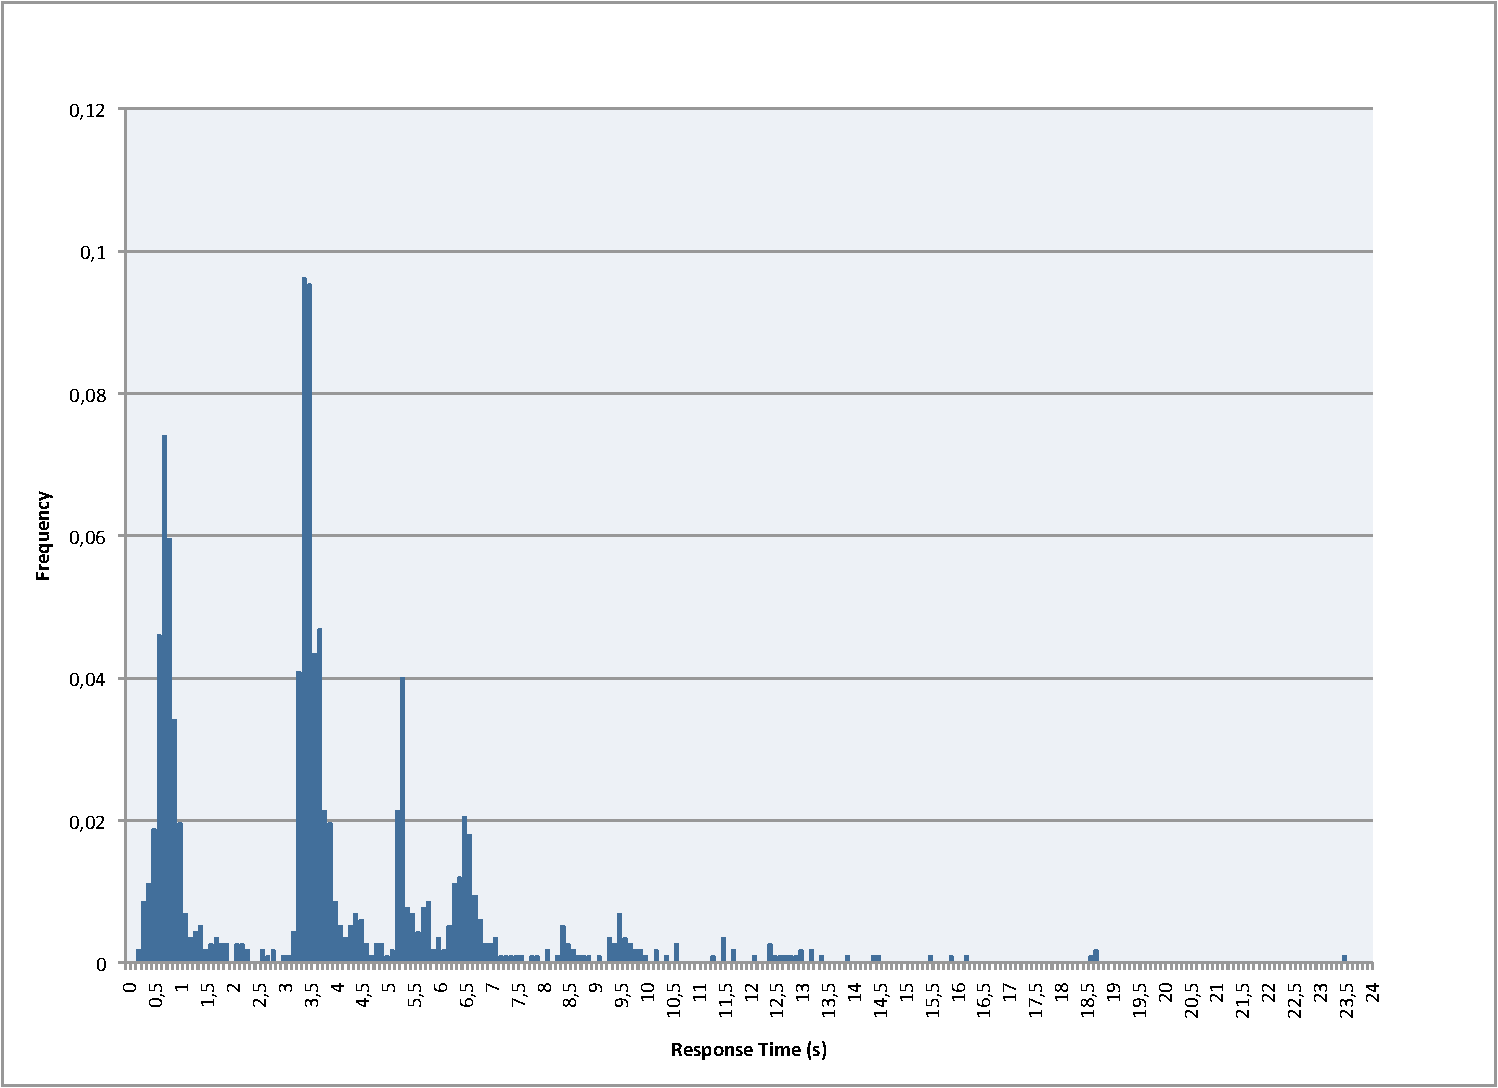
\includegraphics[scale=0.4]{pics/response_time}
\caption{Histogram showing the response time of the server without caching}
\label{fig:response_time}
\end{figure}

We get a mean response time of 3.7 seconds with a standard deviation of 2.8 seconds, but when we look at the histogram we can clearly see a succession of Gaussian distributions, so those values are not really representative of the response model. If we look at the response time over time (Figure \ref{fig:response_time_overtime}) we can see that there are plateaux in the curve.\\

After investigation, it appears that each plateau corresponds to the number of retries that are necessary on the server side to access Västtrafik's data.\\

\begin{figure}[ht]
\center
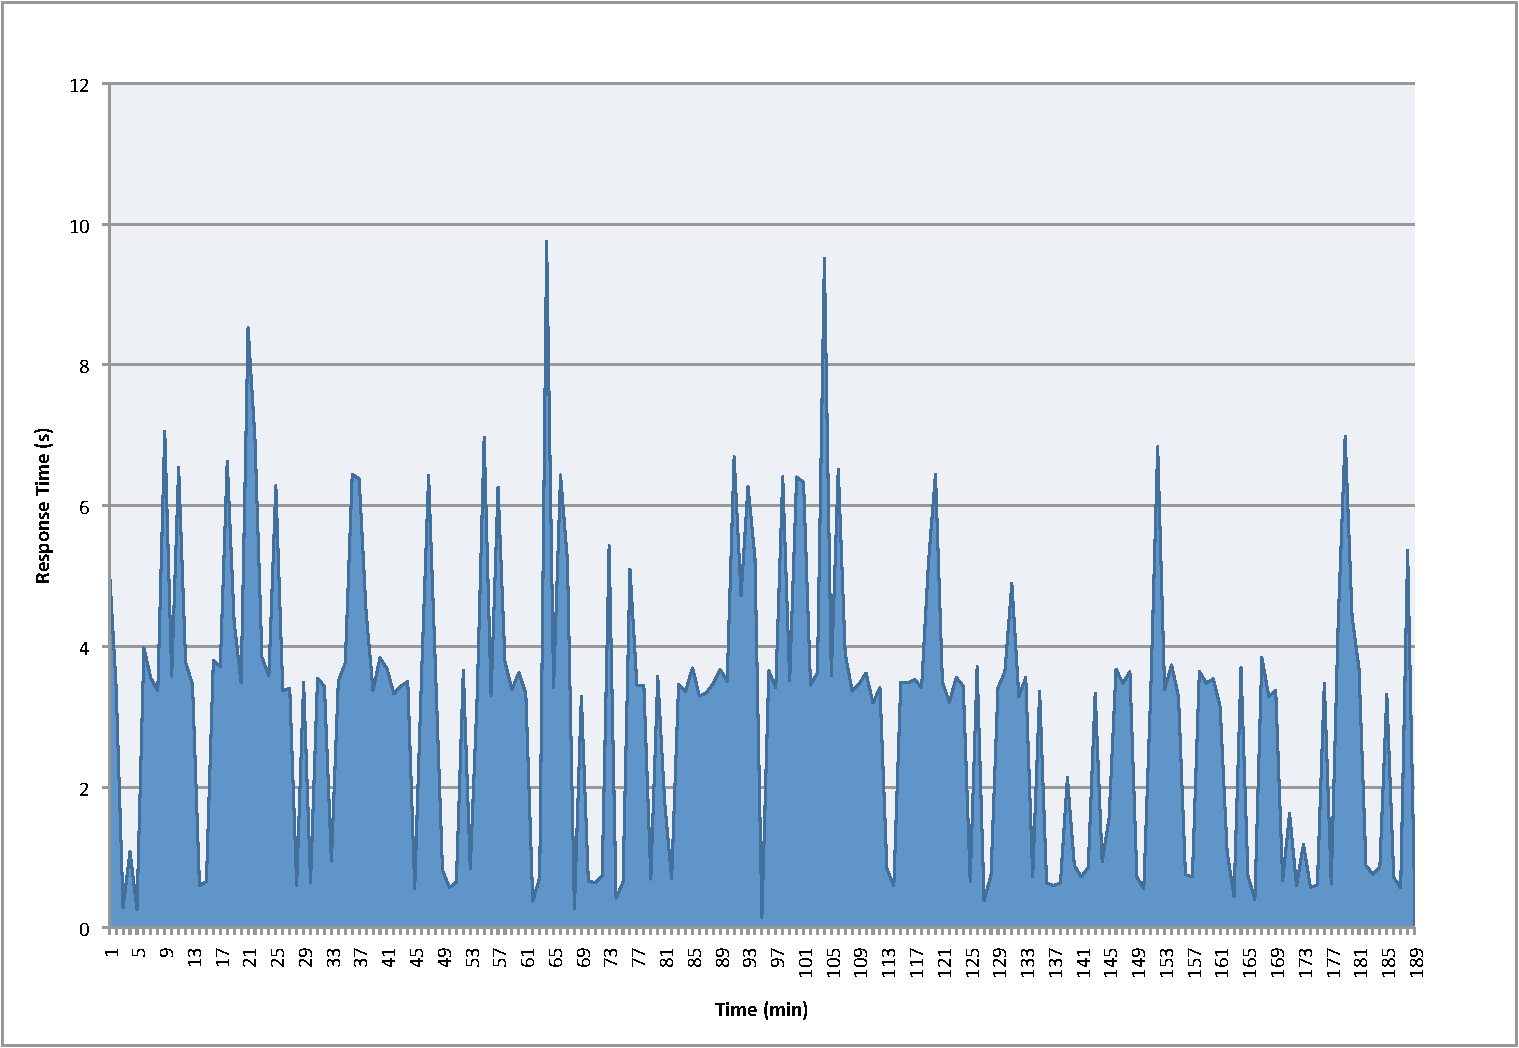
\includegraphics[scale=0.35]{pics/response_time_overtime}
\caption{Response time over time}
\label{fig:response_time_overtime}
\end{figure}

With further considerations, we deduced that when a request is made from Västtrafik and the data is cached on Västtrafik side, the response time gets around 0.6 seconds. When a request is made and the data is not cached on Västtrafik side, the response time gets around 3.5 seconds. This correspond to the two lower plateaux and the first two Gaussian pikes of the histogram in Figure \ref{fig:response_time}. Each higher plateau correspond to a number of retries that are necessary on the server side to access Västtrafik's data. When Västtrafik's servers are overloaded, time-outs and errors can occur thus requiring multiple retries.\\

After getting those results, we also analysed the response time when the data retrieved was beforehand cached by our server. To do so, we sent several requests successively at the same location within 30 seconds and discarded the first query.\\

\begin{figure}[ht]
\center
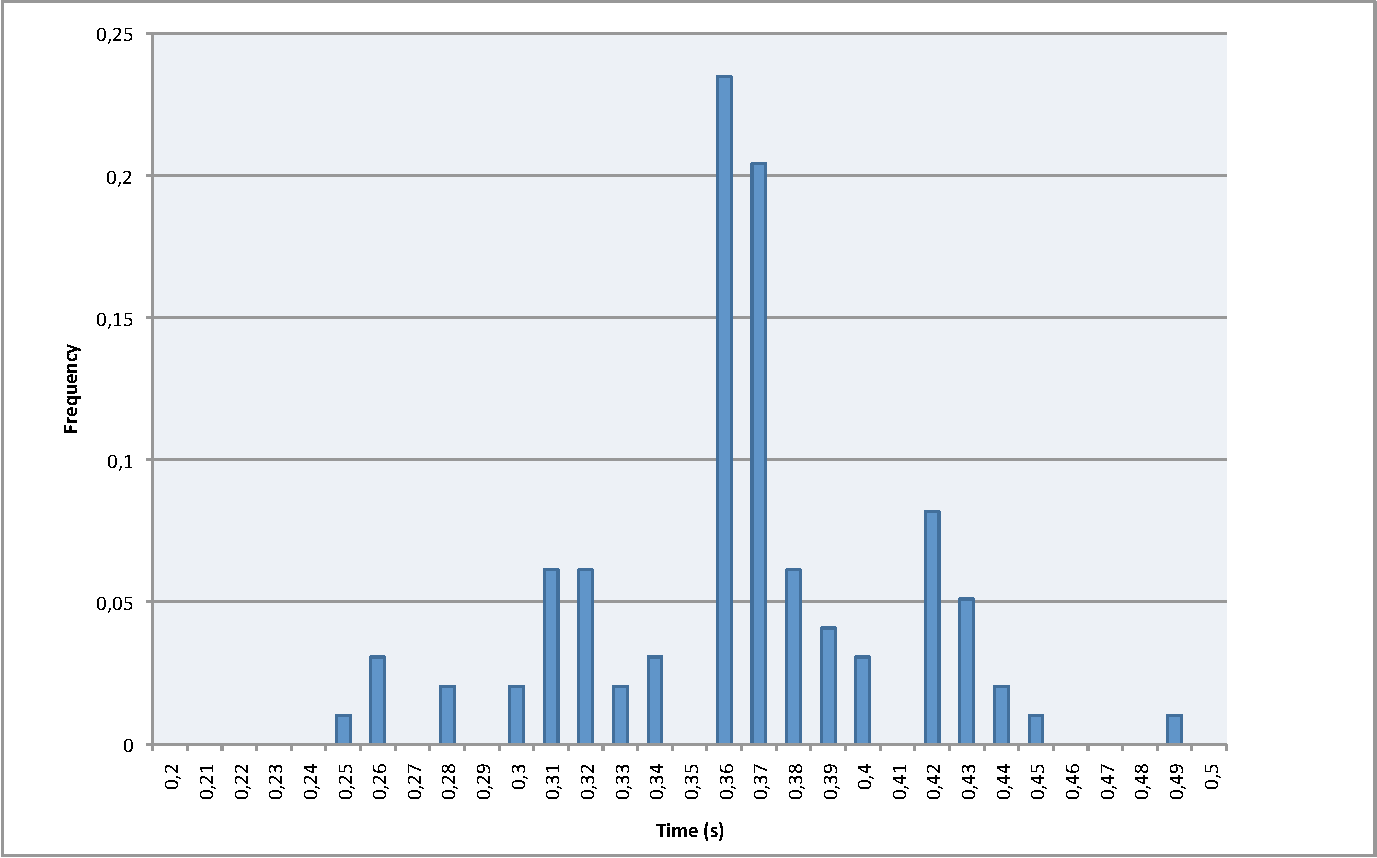
\includegraphics[scale=0.38]{pics/response_time_cached}
\caption{Histogram showing the response time of our server with only cached data}
\label{fig:response_time_cached}
\end{figure}

The result is shown in Figure \ref{fig:response_time_cached}. We get an average response time of 360ms and a standard deviation of 43ms. When looking at the histogram, we see that the distribution is close to a Gaussian distribution, so those values are representative.
